\documentclass[twocolumn,conference]{article}

\usepackage{amsmath,amssymb,amsfonts}
\usepackage{xcolor}
\usepackage{listings}
\usepackage{inputenc}
\usepackage{graphicx}
\usepackage{authblk}
\usepackage{enumerate}
\usepackage{caption}

\usepackage{array,booktabs,longtable,tabularx}
\usepackage{ltablex}
\usepackage{wrapfig,lipsum,booktabs}
\usepackage{multirow}

\providecommand{\keywords}[1]
{
  \small	
  \textbf{\textit{Keywords---}} #1
}

\begin{document}
\author[1]{Eric Raphael Huiza Pereyra}
\affil[1]{Pontifical Catholic University of Peru}
\affil[]{\textit{eric.huiza@pucp.edu.pe}}

\author[2]{Cesar Augusto Olivares Poggi}
\affil[2]{Pontifical Catholic University of Peru}
\affil[]{\textit{cesar.olivares@pucp.edu.pe}}

\title{%
	\vspace{-2.0cm}
	\textbf{Talking with signs} \\	
	\Large \textbf{A method for progressively detect signs in a non annotated signs language corpus}
}

\maketitle
    
\begin{abstract}
People with deafness or hearing disabilities who aim to use computer based systems relies on state of art video classification and human action recognition techniques that combine traditional movement pattern recognition and deep learning techniques. In this work we present a pipeline for semi automatic video annotation applied to a non annotated \textit{Peruvian Signs Language} (PSL) corpus along with a novel method for a progressive detection of PSL elements (nSDm). We produced a set of video annotations indicating signs appearances for a small set of nouns and numbers along with a \textit{labeled PSL dataset} (PSL dataset). A composite model obtained from the combination of a 2D CNN trained with movement patterns extracted from the PSL dataset using Lucas Kanade optical flow, and a RNN with LSTM cells trained with raw rgb frames extracted from the PSL dataset achieved XX precision and XX exhaustivity on sings classification tasks, reporting state of art results over the PSL dataset. \\
\keywords{Video Classification, Human Actions Detection, Peruvian Signs Language, Optical Flow, 2D CNN, LSTM.}
\end{abstract}

\section{Introduction}\label{intro}
The World Health Organization (WHO) stated that 466 million people world wide have disabling hearing loss, estimating that by 2050 over 900 million people will have disabling hearing loss that will represent a global cost of 750 million dollars annually \cite{deafness_and_hearing_loss_2019}. 

The Peruvian Institute of Informatics and Statistics (INEI) conducted a national disabilities survey with the objective of segmenting and acquire a better understanding about disabilities that affect the Peruvian population \cite{disabilities_survey_2012}, the results showed that 1.8\% of the Peruvian population suffer of at least partial when not permanent deafness or hearing limitations. 

With today's Deep Learning techniques for Computer Vision and Natural Language Processing it is completely feasible to propose and design systems that are able to detect and transcribe sign languages elements improving in systems accessibility for people with physical limitations. Sings detection is usually a supervised learning task that requires a large and fully labeled dataset in order to achieve satisfactory results during model training and inference tasks. At the time  of writing this work there were no labeled data sets available for the PSL \cite{lsp_2015}, previous work was done by the \textit{Grammar and Signs research group of the Pontifical Catholic University of Peru (PUCP)} who created the first PSL corpus \cite{lsp_dataset}, this corpus is not annotated because there is no available metadata that describes signs being emitted and

  on annotating a Peruvian Sign Language (PSL) \cite{lsp_2015} a dataset, configuring an expensive and difficult task to achieve. The Pontifical Catholic University of Peru (PUCP) Grammar and  Signs research group created a non annotated PSL dataset \cite{lsp_dataset} because it does not show exactly the relation between the instant when a sign that is emitted and its corresponding translation.

Furthermore, in the same way as spoken languages, signs languages also present local variations e.g. people who live in Lima metropolitan area are not expected to use the same set of signs as people leaving in other parts of the country. A need exists for approaching this task with self-supervised learning or by means of weakly or nonexistent labeled data.

This work reports research conducted with the goal of proposing a method for detecting PSL elements using a not annotated dataset, and answering the following research questions:

\begin{enumerate}[(i)]
\item What are most relevant and currently available techniques for training an AI model from not annotated videos and audio transcription?\label{q1}
\item How precise and exhaustive is the model described in the above question on the recognition of a reduced set of signs in a not annotated dataset?\label{q2}
\item What is the relation between the number of samples and the detection of new LSP elements in terms of nSDm precision and recall?\label{q3}
\end{enumerate}

nSDm will take advantage of the PSL dataset \cite{lsp_dataset} and will contribute with the generalization and progressive signs detection that could be used as a starting point for future studies including software accessibility improvements and human computer interaction for people with deafness and hearing limitations.

The rest of the article is organized as follows. In sec \ref{relatedwork} we review the related work on video classification and body actions recognition using both Optical Flow+Two Stream CNN and 3D CNN architectures. In sec \ref{method} we introduce nSDm and specify its architecture and design. In sec \ref{experimentation} we evaluate nSDm precision and recall and provide answers for the research questions \ref{q1},\ref{q2},\ref{q3}. In sec \ref{datasetdesc} we describe and provide the dataset details. In sec \ref{videoannot} we describe the video annotation and data pre-processing techniques applied to the dataset and finally in sec \ref{conclusion} we present our conclusion and describe future work.
\section{Related Work} \label{relatedwork}
\subsection{Action Recognition}
Human action recognition is a extensively studied field, action recognition dataset like UCF101, HMDB51, THUMOS14  are available, researches tried to solve the human action recognition problem using different approaches including Optical Flow and 3D CNN \cite{qiu2017learning}.  \textbf{Optical Flow,} is defined as the pattern obtained from the motion of objects, surfaces and edges in a visual scene caused by the relative motion between the observer and a scene, it is achieved by distributing movement velocities and brightness across frames. It is a  key concept in action recognition from videos \cite{wang2019hallucinating}. Optical flow estimation is treated as an image reconstruction problem. Given a frame set, the optical flow is generated and allows to reconstruct one frame from the others \cite{zhu2018hidden}. Formally, taking the optical flow displacement field as input and training a CNN with it, then the network should have learned useful representations of the underlying motions. Even though Optical Flow represents the movement between a set of frames, if camera motion is considered as an action motion, it may corrupt the action classification \cite{wang2013dense}. Various types of camera motion can be observed in realistic videos, e.g., zooming, tilting, rotation, etc. \textbf{Motion Boundary Histogram (MBH),} It is a simple an efficient way to achieve robustness during human action detection when camera movements are mixed within the recorded actions by computing derivatives separately for the horizontal and vertical components of the optical flow. Since MBH represents the gradient of optical flow, locally constant camera motion is removed and information about changes in the flow field is kept. MBH is more robust to camera motion than optical flow, thus more discriminative for action recognition.\cite{wang2013dense}. 3D CNN are not as effective as optical flow to detect human actions on its own, 3D CNN can be trained to learn optical flow so we can avoid costly computation and storage and obtain task-specific motion representation  \cite{zhu2018hidden} and increase models performance, precision and exhaustiveness on human action recognition.
\subsection{Pose Estimation}
Pose estimation is also an extensively studied field. Techniques based on key points have shown state of art results on human pose estimation. An approach on key points estimation \cite{tulsianiMalik} uses \textit{Point of View Determination} and \textit{Key Points Prediction} components. Point of View Determination is formulated by the prediction of three Euler angles (azimut, elevation and cyclotation) generating a global position estimate, then a local appearance is modeled by obtaining a heat map that corresponds to the verisimilitude spatial distribution for each key point, finally key points predictions are obtained by combining heat maps obtained in a previous stage with a conditioned verisimilitude at the point of view predicted in the previous stage.

Key points detection methods based CNNs have received an special attention in Human Pose Detection problems, CNNs methods are divided in bottom-up and top-down. Bottom-up methods process images from low resolution  to high resolution, focusing first on detecting joints and then before associating them to human actions. Top-down methods process focused first on detecting humans and then estimating the human pose to predict key points. 

The datasets MPII and COCO have been used in state of art methods obtaining good results\cite{XiaoWuWeiSimpleBaseline} and establishing a framework for future work in combination with classic approaches like optical flow for recognizing patterns movement between frames by increasing accuracy on key points detection.
\subsection{Video Classification}
\textbf{Bag of Words (BoW)} or \textbf{Bag of Visual Words (BoVW)} based on natural language processing techniques is one of the simplest and oldest local descriptor encoding strategies. In its simplest form, it consists of (i) clustering with k-means a collection of descriptor vectors from the training set to build so-called visual vocabulary, (ii) as signing each descriptor to its nearest cluster center from the visual dictionary, and (iii) aggregating the one-hot assignment vectors via average pooling \cite{wang2019hallucinating}, when applied to Computer Vision is a technique used to create images representations or features vectors used that can be learned by CNNs, resulting on improved images classification and video classification. 
Feature trajectory detection are much improved using statistical methods like \textbf{Fisher Vectors} obtaining better results over traditional BoW \textbf{Fussing parallel CNN.}, the Bag of Visual Words representation suffers from sparsity and high dimensionality, in the other hand representations obtained using the Fisher Vectors kernel are more compact and dense which results on better results on image and video classification problems.
\section{Method}\label{method}
\subsection{Video Annotation}\label{videoannot}
The PSL dataset is weakly annotated because there is not a direct relation between the instant when a sign is emitted and when its translation to Spanish is delivered, nSDm proposes a semi automatic video annotation pipeline described in Figure \ref{fig:video-annotation-pipeline} for cleaning, pre-processing and analyzing PSL videos in order to produce an annotated PSL dataset that can be used for training the nSDm model using supervised learning. The pipeline is described in detail in \ref{manual-video-cleanup}, \ref{video-pre-processing}, \ref{audio-transcription-analysis} and \ref{samples-generation}

\begin{figure}[hbt!]
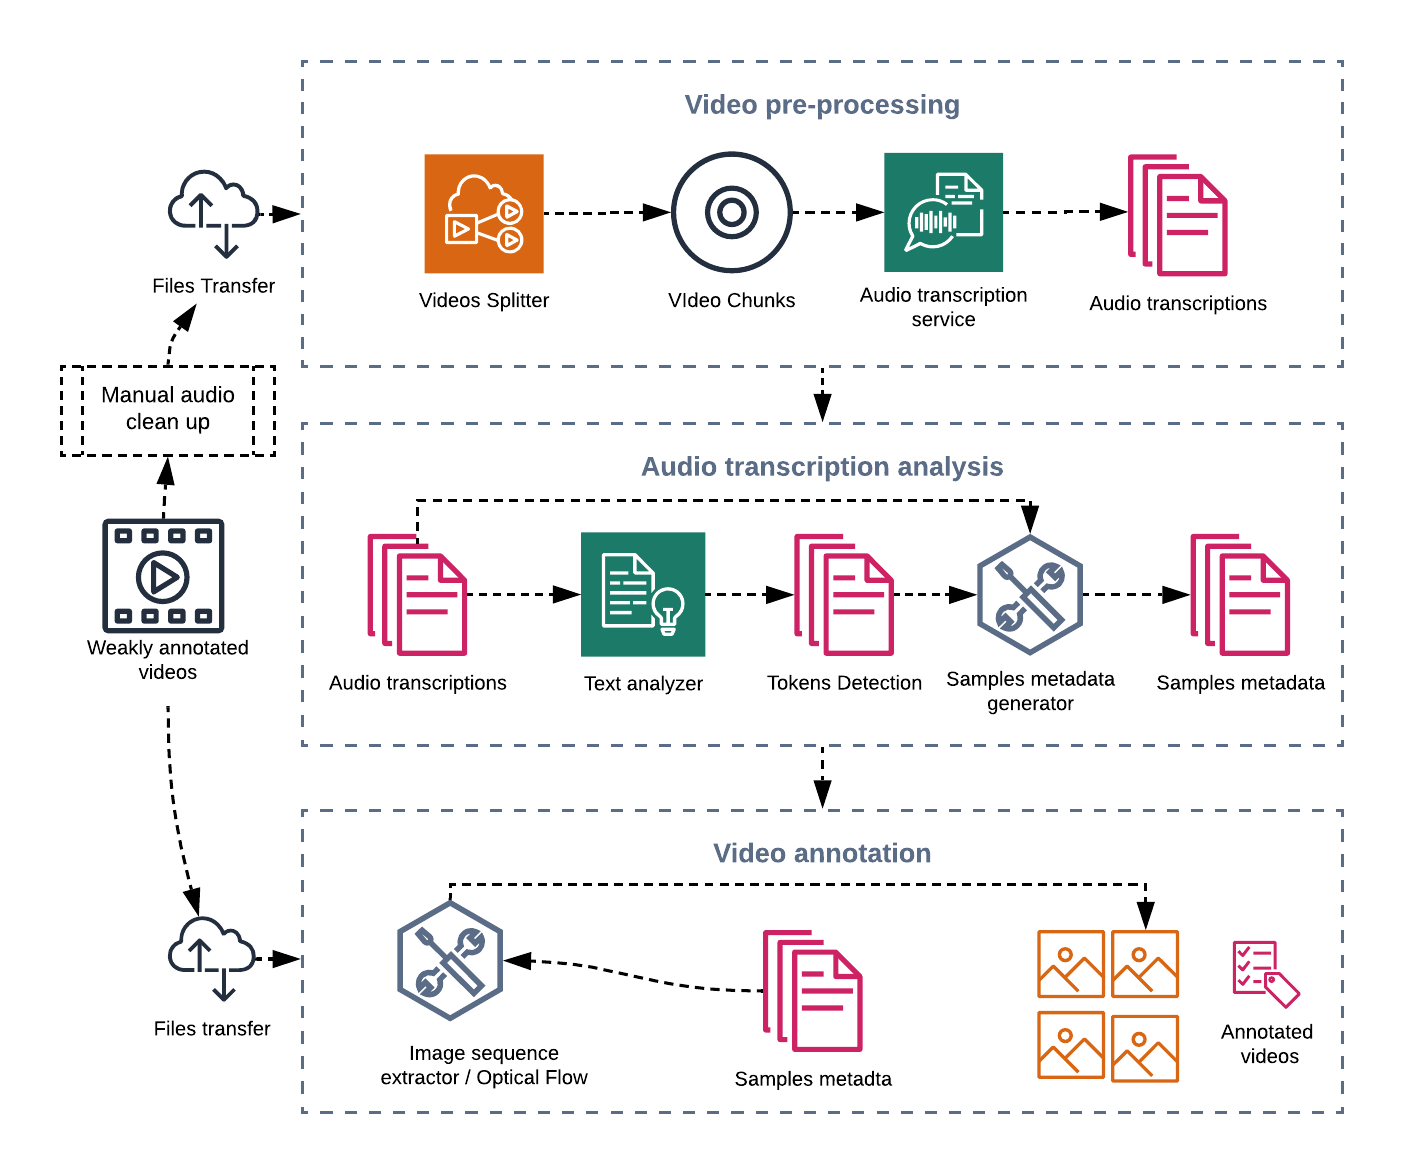
\includegraphics[width=\linewidth]{images/video-annotation-pipeline.png}
\caption{Video annotation process}
\label{fig:video-annotation-pipeline}
\end{figure}

\subsubsection{Manual Automatic Video Clean Up}\label{manual-video-cleanup}
The PSL recordings described on \ref{datasetdesc} contain a considerable amount of noise introduced during the recording sessions which makes difficult to easily find video intervals that clearly show a relation between signs emitted by the informant and the translation delivered by the translator, the noise factors are listed in the following list:
\begin{itemize}
	\item Multiple participants speaking during the session.
	\item Conversations between participants that are not relevant to emitted sings.
	\item High frequency of silent periods.
\end{itemize}
A manual video cleanup process is required to find noise free video intervals, it is a manual process that requires watching all the videos available in the PSL dataset and manually annotating the instant when an informant started emitting sings and the instant when the translator completed delivering a translation, table \ref{table:noise-free-video-segments} shows an annotation example. 

The recordings show the informant in two alignments (centered and left), the manual video clean up process also stores the informant alignment, table \ref{table:informant-alignment} shows the two available alignments, we use the alignment annotation later in the process during the video frames extraction to create the PSL annotated dataset.

% Noise free video segment extract table
\begin{table}[!htb]
\captionsetup{font=footnotesize}
\centering
\begin{tabular}{lrrc}
\toprule
\multicolumn{1}{c}{\textbf{Video}} & 
	\multicolumn{1}{c}{\textbf{Start}} &
	\multicolumn{1}{c}{\textbf{End}} &
	\multicolumn{1}{c}{\textbf{Alignment}}\\
\midrule
\multirow{5}{7.5em}{\textbf{consultant-01-session-01-part-01.mp4}} & 00:30 & 00:55 & center\\
& 01:15 & 01:29 & center\\
& 00:53 & 01:07 & center\\
& 08:12 & 09:01 & center\\
\midrule
\multirow{5}{7.5em}{\textbf{consultant-02-session-01-part-01.mp4}} & 00:15 & 00:21 & center\\
& 00:15 & 00:21 & center\\
& 00:53 & 01:07 & center\\
& 02:43 & 02:47 & center\\
& 17:33 & 18:01 & left\\
\bottomrule
\end{tabular}
\captionsetup{font=footnotesize}
\caption{Noise free video segments extract} \label{table:noise-free-video-segments}
\end{table}

% Informat aligment
\begin{table}[!htb]
\captionsetup{font=footnotesize}
\centering
\begin{tabular}{cc}
\toprule
\multicolumn{1}{c}{\textbf{Center Aligned}} & 
	\multicolumn{1}{c}{\textbf{Left Aligned}}\\
\midrule
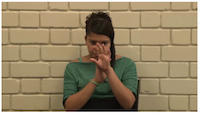
\includegraphics{images/informant-center-alignment.png}& 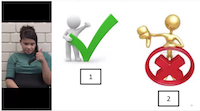
\includegraphics{images/informant-left-alignment.png}\\
\bottomrule
\end{tabular}
\caption{Informant Alignment} \label{table:informant-alignment}
\end{table}

\subsubsection{Video Pre-Processing}\label{video-pre-processing}
Weakly PSL annotated videos require processing before any metadata can be extracted, we propose a sequence of pre-processing tasks that take advantage of the annotation generated on \ref{manual-video-cleanup}. A \textbf{video splitting processor} generates a set of video chunks using the \textit{ffmpeg} multimedia framework and stores the produced chunks in Amazon S3 for later usage. The audio within the video chunks is then transcribed by an \textbf{audio transcription processor}, using the Amazon Transcription service, we selected the Amazon Transcription service because it provides an accurate mapping between audio participants and transcribed words along with useful metadata that describes the start and end time when words are pronounced. 

At the moment of writing this work Amazon Transcription service only supported Spanish for Spain and the US, it caused certain words that are specific for Peruvian Spanish not being fully recognized, in order to improve transcription accuracy we provided a custom vocabulary containing Peruvian expressions which improved  Peruvian words recognition, for the matters of this work unrecognized Peruvian words were omitted and not processed.

\subsubsection{Audio Transcription Analysis}\label{audio-transcription-analysis}
Audio transcription requires additional processing in order to produce useful information that leads to a successful PSL signs detection. Bag of Embedding Words (BoEW) is a widely used technique on Natural Language Processing tasks providing a easy and flexible way to list the most relevant words based on frequency. This work is focused on detecting nouns and numbers (nSDm is a ongoing method that will be progressively improved to handle a wider set of PSL elements) assuming that nouns (numbers are a subset of nouns) suffer less variations in spoken Spanish than verbs, pronouns, adverbs and adjectives, and provide more semantic value than conjunctions, prepositions and interjections. 

\begin{table}[!htb]
\captionsetup{size=footnotesize}
\begin{tabular}{ p{16em} c}
\toprule
\multicolumn{1}{c}{\textbf{Token}} & 
	\multicolumn{1}{c}{\textbf{Frequency}}\\
\midrule
\textbf{pareja}&	40\\
\textbf{cosas}&	30\\
\textbf{cine}&	20\\
\textbf{noche}&	20\\
\textbf{terror}&	10\\
\textbf{parque}&	10\\
\textbf{casa}&	10\\
\textbf{montón}&	10\\
\textbf{apariciones}&	10\\
\textbf{fantasmas}&	10\\
\textbf{dos}&	10\\
\bottomrule
\end{tabular}
\caption{Most relevant tokens detection frequency in the PSL dataset} \label{tab:token-freq}
\end{table}

We used Amazon comprehend for text analysis, specifically the syntax detection functionality which will provide a comprehensive list of detected language elements along with a score from 0.0 to 1.0 indicating the detection accuracy, we have selected the ones that have at least a 0.8 accuracy score and omitted the rest, this process was automated using a \textbf{transcription detection processor} which uses BoEW to provide a list of most relevant nouns and numbers based on appearance frequency. Table \ref{tab:token-freq} shows a list of nouns and numbers and their frequencies in the PSL dataset.

Once a weighted list of nouns and numbers is generated a mapping showing when nouns and numbers appear in videos is required, moving forward called \textbf{Samples Metadata}. Table \ref{tab:token-video-mapping} shows mapping metadata extracted from PSL.

\subsubsection{Samples Generation}\label{samples-generation} 
nSDm requires PSL elements to be represented as a set of RGB frames and a calculated Optical Flow using the Lucas-Kanade method, both representations are inputs of two different models as presented on \ref{nsdm}.

\textbf{Translation Delay Factor: } The difference in time between the instant when a sign is emitted and when a translation for that given sign is delivered is uncertain, we are calling that uncertainty as the \textit{translation delay factor} which we are trying to approximate using a constant value, we have chosen a 3 seconds translation delay factor assuming that most of the translations will occur between three seconds after a sign is emitted.

A \textbf{RGB Samples generation processor} uses samples metadata in combination with the translation delay factor to determine frames that represent a given PSL element. We use \textit{OpenCV} to extract frames and store them following a hierarchical folder structure (listing \ref{list:rgb-samples-folders}) that nSDm data loaders will use to feed data into the RGM branch on the nSDm model architecture during training and testing.

A \textbf{Optical Flow Samples generation processor} uses video frames and the hierarchical folder structure generated by the RGM samples generation processor to calculate an Optical Flow representation for PSL elements and store them in a hierarchical folder structure that will also used by the nSDm data loaders to feed the optical flow branch on the nSDm model architecture during training and testing. We selected optical flow as a samples generation strategy because its ability to represent movement traces from previous frames, it is particular useful for representing PSL elements, a PSL element is composed on different body movements including: elbow, arms, neck, eyes, shoulders and hands, which are performed quickly, a way to detect movement traces between frames allows to generate a single image representation of all movement involved on a sign emitting (Figure \ref{fig:opticalflow-two}). 

\begin{table}[!htb]
\captionsetup{font=footnotesize}
\centering
\begin{tabular}{ l p{10em} r r }
\toprule
\multicolumn{1}{c}{\textbf{Token}} & 
	\multicolumn{1}{c}{\textbf{Video}} &
	\multicolumn{1}{c}{\textbf{Start}} &
	\multicolumn{1}{c}{\textbf{End}}\\
\midrule
\textbf{cine}&	consultant-02-session-01-part-01-00.mp4&	4.19&	4.75\\
\textbf{cine}&	consultant-02-session-01-part-01-01.mp4&	1.19&	1.75\\
\textbf{terror}&	consultant-02-session-01-part-01-01.mp4&	3.82&	4.4\\
\textbf{parque}&	consultant-02-session-01-part-01-03.mp4&	8.97&	9.3\\
\textbf{casa}&	consultant-02-session-01-part-01-03.mp4&	10.12&	10.57\\
\textbf{pareja}&	consultant-02-session-01-part-01-04.mp4&	3.91&	4.36\\
\textbf{noche}&	consultant-02-session-01-part-01-04.mp4&	4.49&	4.92\\
\textbf{noche}&	consultant-02-session-01-part-01-04.mp4&	7.91&	8.2\\
\textbf{mont\'on}&	consultant-02-session-01-part-01-04.mp4&	8.5&	8.78\\
\textbf{cosas}&	consultant-02-session-01-part-01-04.mp4&	8.88&	9.38\\
\bottomrule
\end{tabular}
%\end{tabular}}
\caption{Shows metadata extacted from the PSL dataset: (1)\textit{Token} could be a noun or a number (2)\textit{Video Path} shows the video where the token was detected (3)\textit{Start Time} time when the token reproduction starts (4)\textit{End Time} time when the token reproduction ends.}
\label{tab:token-video-mapping}
\end{table}

\subsection{Novel Signs Detection Method (nSDm)}\label{nsdm}
\subsubsection{Architecture}\label{nsdm-architecture}
\begin{figure}[hbt!]
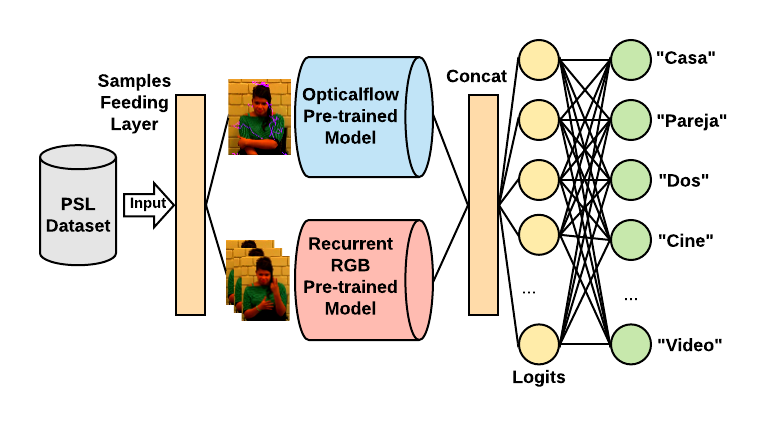
\includegraphics[width=\linewidth]{images/composite-model-architecture.png}
\caption{nSDm model architecture}
\label{fig:opticalflow-two}
\end{figure}

\begin{figure}[hbt!]
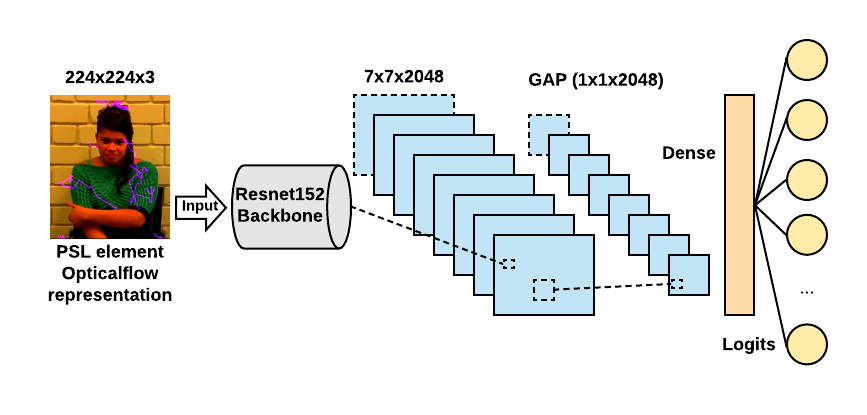
\includegraphics[width=\linewidth]{images/opticalflow-model-architecture.png}
\caption{Opticalflow model architecture}
\label{fig:opticalflow-two}
\end{figure}

\begin{figure}[hbt!]
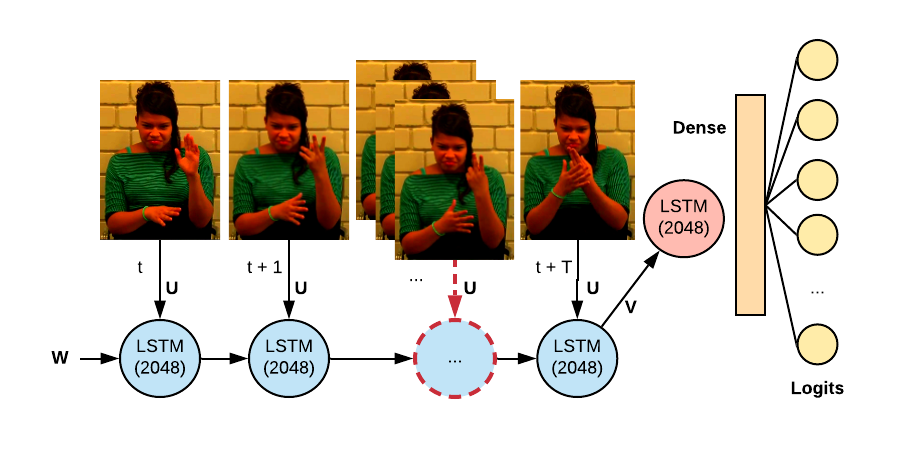
\includegraphics[width=\linewidth]{images/recurrent-rgb-model-architecture.png}
\caption{Recurrent RGB model architecture}
\label{fig:opticalflow-two}
\end{figure}

\subsection{New Videos Testing}

\section{Experimentation}\label{experimentation}
\subsection{Dataset Description \cite{lsp_dataset}}\label{datasetdesc}
The PSL dataset was developed by the PUCP Grammar and Signs research group in 2014 and consists in a set of videos recorded during the interviews of 24 individuals, 12 male and 12 female informants, all of them are Lima Peru residents and reported to be borne with a permanent deafness condition or acquired the condition before the acquisition of Spanish. 

The dataset consists in 718 video clips recorded with a ADR-CX220 SONY HD camera which included an embedded microphone. The camera focused only the informant but also recorded questions, instructions and translations.

The video clips were recorded in three sessions with the following participants: A coordinator, a PSL \cite{lsp_2015} translator and a informant.\\

\textbf{Recording Session 1}: A 45-60 minutes semi structured interview that included: Biographic information as well as habits, anecdotes, opinion about cultural subjects and elicitation of names, states and actions. 

\textbf{Recording Session 2}: The informant was presented with a set of 55 cards describing actions and were asked to choose a set of them in order to build a coherent story that was subsequently told by the informant.

\textbf{Recording Session 3}: A PSL \cite{lsp_2015} conversation facilitated by the coordinator happening between the informant and the translator.\\

During all the sessions a PSL \cite{lsp_2015} translator performs a translation after a word or phrase is completed.

\subsection{Video Annotation Results}
The video annotation pipeline described on \ref{videoannot} produced an annotated PSL dataset suitable for using it in a supervised learning experiment. The annotated dataset is divided in two main parts (RGB and Optical Flow samples)

\textbf{RGB Samples folder structure} is a hierarchical folder structure where each detected noun or number is represented as a first level folder, all instances of a detected sign received an identifier which is an auto incremental integer, detected instances represent the second level folders, detected signs video represent the third level, Figure \ref{fig:rgb-two}.
\begin{lstlisting}[caption=RGB Samples Folder Structure example, basicstyle=\ttfamily\small]
L1:dos
	L2:1
		L3:rgb-frame01.jpg
		L3:rgb-frame02.jpg
		L3:rgb-frame03.jpg
		...
		L3:rgb-frame08.jpg
L1:cine
	L2:1
		L3:rgb-frame01.jpg
		L3:rgb-frame02.jpg
		L3:rgb-frame03.jpg
		...
		L3:rgb-frame15.jpg
	L2:2
		L3:rgb-frame01.jpg
		L3:rgb-frame02.jpg
		L3:rgb-frame03.jpg
		...
		L3:rgb-frame11.jpg
\end{lstlisting}\label{list:rgb-samples-folders}

\begin{figure}[hbt!]
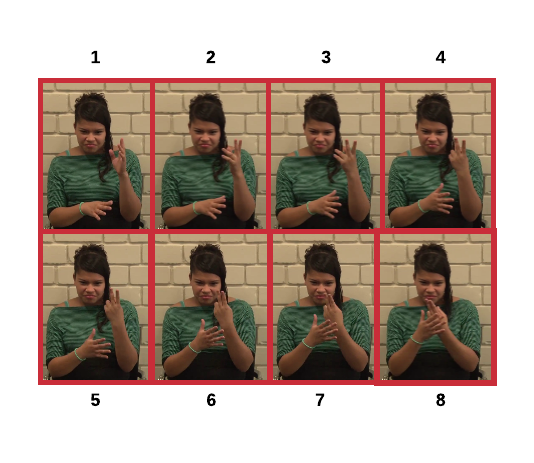
\includegraphics[width=\linewidth]{images/dos-rgb-frames.png}
\caption{PSL number "Two" RGB representation}
\label{fig:rgb-two}
\end{figure}

\textbf{Optical Flow samples folder structure} is a hierarchical folder structure based on the RGB samples folder structure, it is a more simple based on two levels instead of three, the nature of Optical Flow of tracing movement between frames allow to produce a single image for each detected PSL element instance (listing \ref{list:opticalflow-samples-folders}), Figure \ref{fig:opticalflow-two} shows an example of an optical flow generated sample
\begin{lstlisting}[caption=Optical Flow Samples Folder Structure example, basicstyle=\ttfamily\small]
L1:dos
	L2:oflow-dos-01.jpg
L1:cine
	L2:oflow-cine-01.jpg
	L2:oflow-cine-02.jpg
\end{lstlisting}\label{list:opticalflow-samples-folders}
\begin{figure}[hbt!]
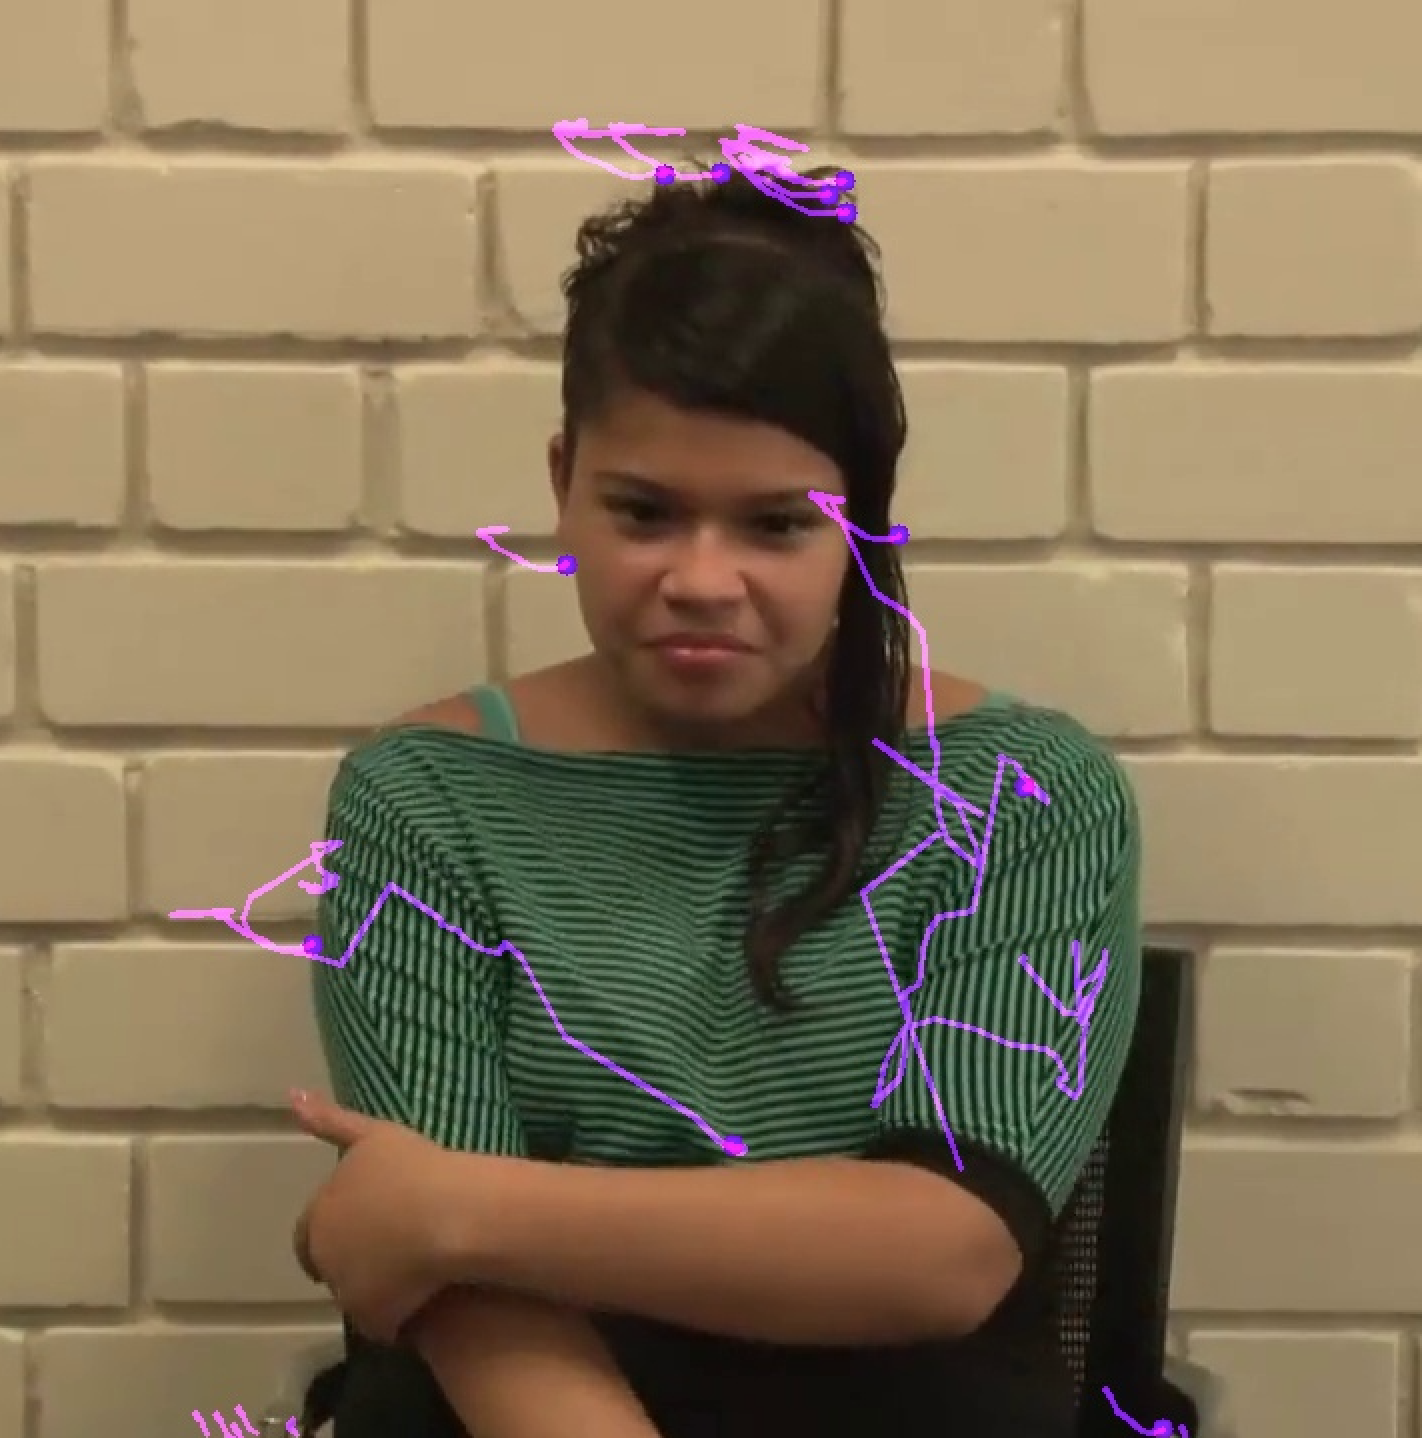
\includegraphics[width=\linewidth]{images/dos-opticalflow.jpg}
\caption{PSL number "Two" OpticalFlow representation}
\label{fig:opticalflow-two}
\end{figure}

\subsection{nSDm results}

\section{Conclusion}\label{conclusion}

\bibliographystyle{ieeetr}
\bibliography{References}


\end{document}
